\chapter{WPA2-PSK secured WiFi network attack}
\label{app:wifi_attack}

In the following example, we seek to compromise a WiFi encrypted network, since WiFi networks are commonly used for the transport layer in IoT architectures.

\begin{figure}[htbp]
	\centerline{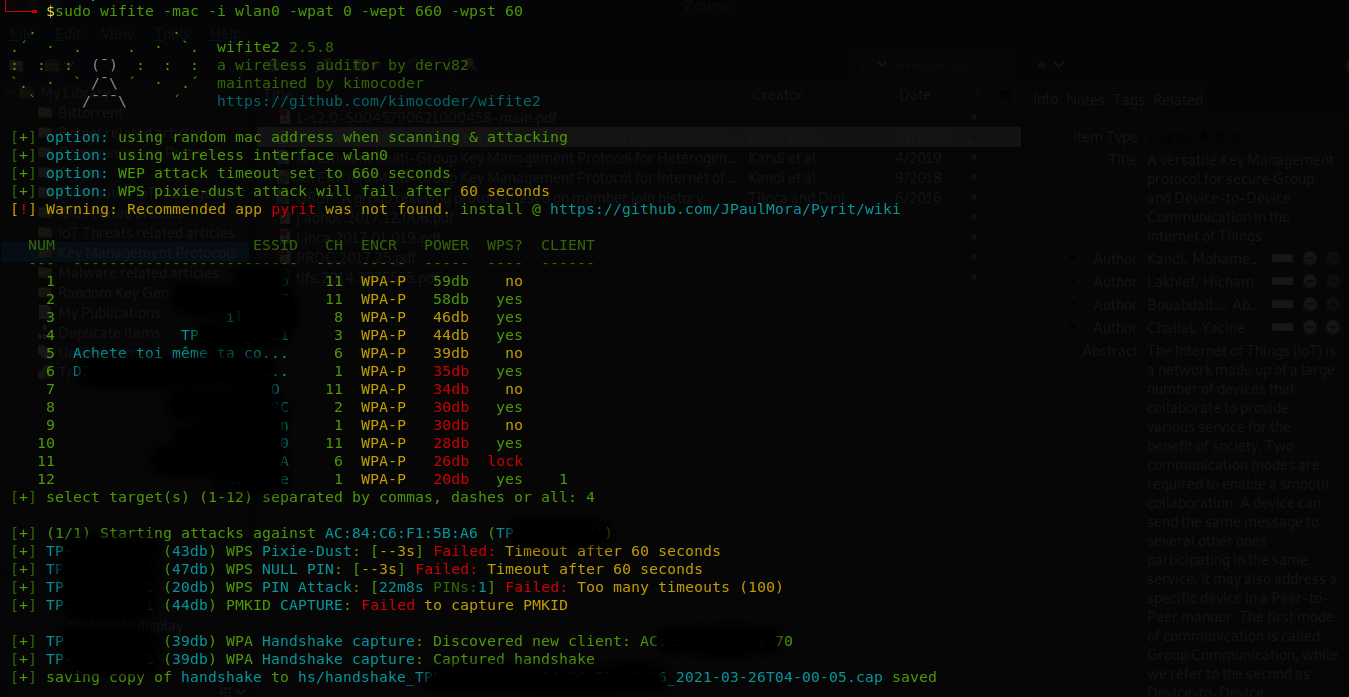
\includegraphics[scale=0.25]{figures/wifi/wifite1bis.png}}
	%\caption{Election procedure}
	\label{fig}
\end{figure}

The first step is to technically identify the WiFi AP through ots ESSID and BSSID. The objective is to dump a handshake exchange with one client. If we can manage to identify a connected client to the network, we can try to cut it off from thr network by sending multiple deauth frames. This will force the client to reconnect to the AP, allowing us to capture the handshake. Once the handshake is captured, we crack it to obtain the WiFi network’s key.

\begin{figure}[htbp]
	\centerline{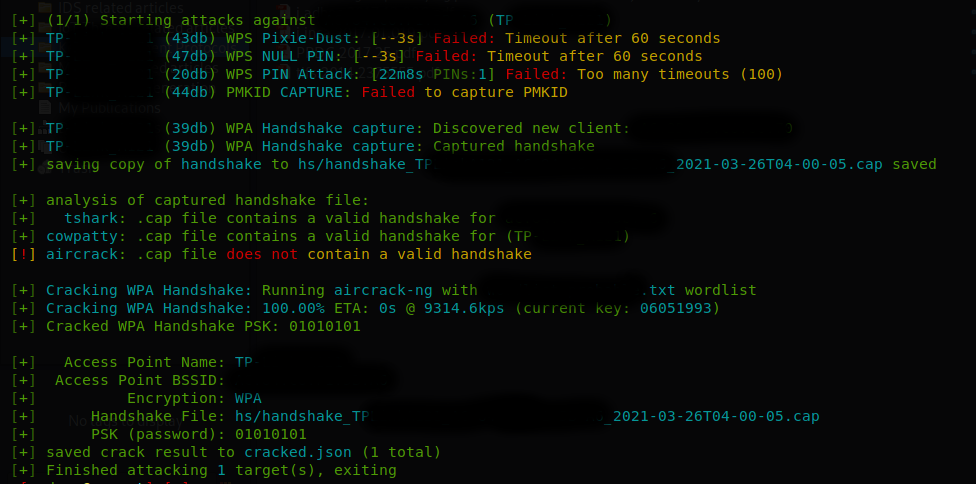
\includegraphics[scale=0.35]{figures/wifi/wifite2bis.png}}
	%\caption{Election procedure}
	\label{fig}
\end{figure}

What we actually do is that we analyse the captured .cap file to extract the password. We use a dictionary-based attack in order to find a match for the captured handshake by replaying the exchange for different possible passwords.

%\begin{figure}[htbp]
%	\centerline{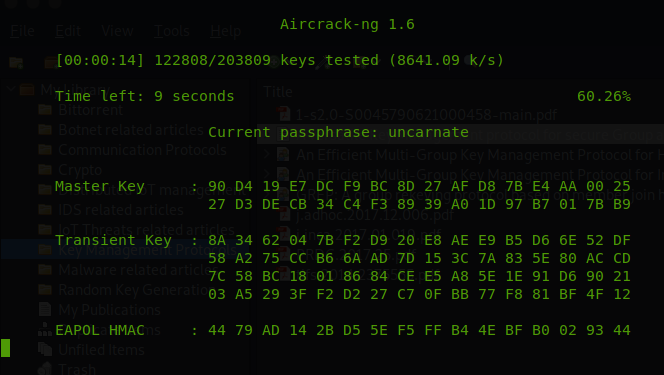
\includegraphics[scale=0.45]{figures/wifi/aircrack1.png}}
	%\caption{Election procedure}
%	\label{fig}
%\end{figure}

Using a dictionary-based password attack, we are able to recover the password in just few seconds.

\begin{figure}[htbp]
	\centerline{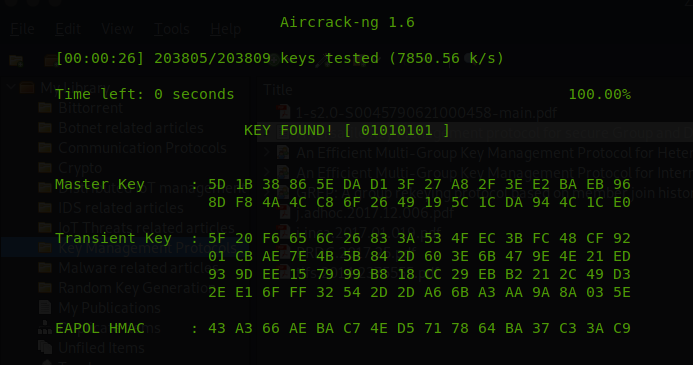
\includegraphics[scale=0.50]{figures/wifi/aircrack2.png}}
	%\caption{Election procedure}
	\label{fig}
\end{figure}